% This is samplepaper.tex, a sample chapter demonstrating the
% LLNCS macro package for Springer Computer Science proceedings;
% Version 2.20 of 2017/10/04
% TEMPLATE: https://www.springer.com/de/it-informatik/lncs/conference-proceedings-guidelines
%
\documentclass[runningheads]{llncs}

\usepackage{graphicx}
\usepackage{todonotes}
\newcommand{\comment}[1]{}

% Used for displaying a sample figure. If possible, figure files should
% be included in EPS format.
%\usepackage{comment}
\newcommand{\comment}[1]{}
%\usepackage{lettrine} % if you want the first letter to be \letterine{b}{igger}
% If you use the hyperref package, please uncomment the following line
% to display URLs in blue roman font according to Springer's eBook style:
% \renewcommand\UrlFont{\color{blue}\rmfamily}

%\newcommand{\rom}[1]{\uppercase\expandafter{\italic\romannumeral #1\relax}}  % roman numbers with \rom{num}
%\newcommand{\ber}[1]{\lowercase\expandafter{\italic #1\relax}} % a
\newcommand{\rom}[1]{\textit{#1}}
\newcommand{\ber}[1]{\textit{#1}}

\newcommand{\reffig}[1]{Figure~\ref{#1}}
\newcommand{\reftab}[1]{Table~\ref{#1}}
\newcommand{\refsec}[1]{Section~\ref{#1}}

\begin{document}
%
\title{Towards private Active Choreographies on public blockchain}
%
%\titlerunning{Abbreviated paper title}
% If the paper title is too long for the running head, you can set
% an abbreviated paper title here
%
\author{Henry Bergstroem\inst{1} \and
Jan Mensch\inst{1, 2}}
%
\authorrunning{F. Author et al.}
% First names are abbreviated in the running head.
% If there are more than two authors, 'et al.' is used.
%

\institute{Hasso-Plattner-Institut, Prof.-Dr.-Helmert-Straße 2-3, 14482 Potsdam, Germany 
\email{	bergstroem@uni-potsdam.de}
\and
University of Potsdam, Am Neuen Palais 10, 14469 Potsdam, Germany  \\
\email{jan.mensch@uni-potsdam.de}}

%
\maketitle              % typeset the header of the contribution
%
\begin{abstract}

    Make it clear that we are talking about an implementation of ACs, not the BPMN standard!
    
    \todo{write abstract}
    
    We are working towards implementing a realization of ACs, that implements some visibility constraints that you would usually see in real-world applications, like confidential data and transactions.

\end{abstract}

\section{Introduction} \label{sec:intro}

Integrating business processes has been found to have a positive impact on the operational and business performance \cite{flynn2010impact,narayanan2011antecedents}. However a lack of trust between business partners is hindering such progress \cite{panayides2009impact}. By proposing a solution that needs neither trust between participants, nor trust in any central authority and keeps the business done secret, we hope to further increase collaboration between businesses. As shown by Weber et al. in \cite{weber2016untrusted}, there are ways to extend the use cases of business process execution and auditing to an untrusted environment, thus making it possible for entities to collaborate with each other that would usually not be willing to do so. This execution of untrusted business processes is made possible by using an blockchain-based implementation \todo{Implementation of ACs, not the modeling standard} of Active Choreographies, which we will briefly discuss in \refsec{subsec:blockchainbased}.\footnote{Phrasing and sources of the Introduction where in part taken from \cite{weber2016untrusted}} 

The goal \todo{Quick motivation. Can this stay in the introduction?} of this paper is to explore the notions of privacy and visibility with regards to untrusted execution of choreographies on the blockchain and to introduce a schema which aims to keep untrusted business process execution \todo{untrusted b.p. execution from Weber. Do I need to define this?} private, while still being enforceable. The structure of the paper is as follows: Introduction (\refsec{sec:intro}).  Background (\refsec{sec:background}), where we will give a short introduction over the work we considered when creating our solution. Approach (\refsec{sec:approach}). An overview of the proposed solution. Evaluation (\refsec{sec:eval}),  where we introduce our implementation. Discussion (\refsec{sec:discussion}). An summary over limitations, alternative implementations and future work and the Conclusion (\refsec{sec:conclusion}).





\todo{if this is too short, bring up blockchain?}


\section{Background} \label{sec:background}

\subsection{Blockchain-Based choreographies} \label{subsec:blockchainbased}

basically a more specific Introduction

what did Ingo do?

what did Jan do?




\subsection{Visibility levels} \label{subsec:levels}

While the issue of privacy was mentioned by Weber et al. and Ladleif, they did not take any measures to actually implement them. However, Latleif did introduce different levels of visibility in the context of modeling business contracts with ACs \cite{ladleif}. The levels are as follows:



\begin{itemize}
    \item \ber{Model level}: The logic of the business process. If you would model a business process using BPMN, the BPMN model would be the model layer. If you would implement it using a programming language, the source code would be the model layer.
    \item \ber{Communication level}: The knowledge of which messages were exchanged, who exchanged them and which entities are part of the business process. Latleif also includes the time at which messages were send. For the scope of this publication, we would like to exclude the time of an exchanged message from the communication level.
    \item \ber{Content level}: The content of the exchanged messages.
\end{itemize}

We are referring to these levels when discussing the assumptions that our approach is based on in \refsec{subsec:assumptions} and also in \refsec{subsec:schema}, when we discuss our proposed solution. \todo{I do not want to repeat the motivation for why we need the levels. Is this ok?}






\subsection{Privacy Enhancing Technologies} \label{subsec:technologies}

\textbf{Privacy Enhancing Technologies on the Blockchain}. Our implementation aims to provide privacy for all three layers. We considered multiple other technologies that are \todo{Do we need to tell the reader why we mention this?} worth mentioning and could be a viable alternative to our approach. \todo{try to be a bit more high-level, not too focused on possible solutions}

One of them is \textit{obfuscation}. This is a technology that "aims to make a computer program 'unintelligible' while preserving its functionality" \cite{garg2016candidate}. Since it was shown in \cite{barak2001possibility,barak2012possibility} that there is a set of functions that are impossible to obfuscate, the idea of indistinguishable obfuscation was introduced. This is a weaker constraint, guaranteeing that it is impossible to distinguish two equivalent programs that have been obfuscated. These ideas seem to be very powerful, but come with a big drawback: Being extremely computationally expensive \cite{banescu2015idea}. \todo{do I need a line break here or can I just write one long paragraph?}

\textit{Homomorphic encryption} might be used to do calculations on encrypted values \todo{source}. Similar to obfusaction, homomorphic encryption suffers from heavy computational overhead \todo{source}.


A further technology considered is \textit{secure multi-party computation (SMPC)} \cite{orlandi2011multiparty}. With SMPC, there are are multiple parties involved in computing the output of a function. These parties do not have to trust each other. They thus need a protocol that makes sure that the output is correct and that cheating participants will not be able to learn anything about the input of the honest parties. \todo{Should we really not tell the reader why we consider this a nice technology for our purpose? Or does all of this go into the Discussion (for all technologies)?}


A technology already in use in blockchain applications are zero-knowledge Succinct Non-interactive ARguments of Knowledge (zk-SNARKs). An application using it is Zerocoin, which aims to provide "fully anonymous currency transactions" \cite{miers2013zerocoin}. zk-SNARKS provide the possibility to have an untrusted prover verify a statement (or secret) made by a different party, without that party having to reveal their secret \cite{ben2013snarks}. It furthermore does so in a non-interactive manner. 



Also already applied in the context of blockchain applications are \textit{Ring Signatures}. This is a signature created using the public keys of multiple parties. It can be used to verify that a message was send by one of the parties, without revealing which of them was the sender. For this the sender "does not need the knowledge, consent, or assistance" of anyone else in the group  \cite{rivest2001leak}. In Monero this technology, together with one-time keys, is used to hide the identity of the sender and the receiver of a transaction  \cite{noether2016ring}.



Today there exist already multiple projects that focus on business process execution \todo{citations of those projects}. Some of them provide mechanisms aiming to create trust between participants \todo{Give example. Explain how they provide that trust?}. A further already existing implementation is  \textit{parity ethereum}. With parity, users are able to hide private contracts in public contracts and to exchange private messages \cite{parity}.

\comment{However for private contract execution parity is relying on validators, "account[s] that can allow a private contract’s state [to] change" \cite{parity}. In our understanding this makes parity insufficient for untrusted business execution, since, like private blockchains, it requires trust in one or multiple nodes. 
}




\section{Approach} \label{sec:approach}

\subsection{Assumptions and Scenario} \label{subsec:assumptions}

Before introducing our schema, we would like to mention the assumptions on which our proposal is based on. Each premise is marked for potential later reference. \todo{do I need this? Am I referring to any of the specific points later on?}



\bigbreak
\textbf{Assumptions about the participating parties}: \ber{a} There are several parties which want to collaborate. These parties have \ber{b} neither trust in each other nor \ber{c} trust in any third party. They furthermore \ber{d} want to keep their business processes secret, \ber{e} hide with whom they are collaborating and \ber{f} hide what messages are exchanged during the collaboration. Since the parties distrust each other they also \ber{g} only want to share messages with the entities that have to see them and keep them secret from the others. Each party \ber{h} is "honest but curious" \todo{cite a reference here}. They follow the protocol, but will try to collect as much information as possible. These assumptions justify that we aim to keep all levels mentioned in \refsec{subsec:levels} \todo{when refering to a subsection, do I have to write subsection x.y?} private. To be more specific, \ber{d} requires a private \ber{Model Level}, \ber{e} a private \ber{Communication Level} and \ber{f} a private  \ber{Content Level}.


\bigbreak
\textbf{Further assumptions:}
\ber{i} All data that is processed on the blockchain is considered public. It is \ber{j} possible to convert a business process into a program or state-machine in order for parties to determine that validity of a state change. \ber{k} In terms of trust, a public blockchain is superior to a private one, since it does not require trust in the organisation that runs the network. \ber{l} A network that employs "policing notes" \footnote{Nodes that have the special role of enforcing rules or similar tasks} is considered inferior to a network without such nodes, since such a network requires "trust in the authorities".



\begin{figure}[h!]
    \centering
    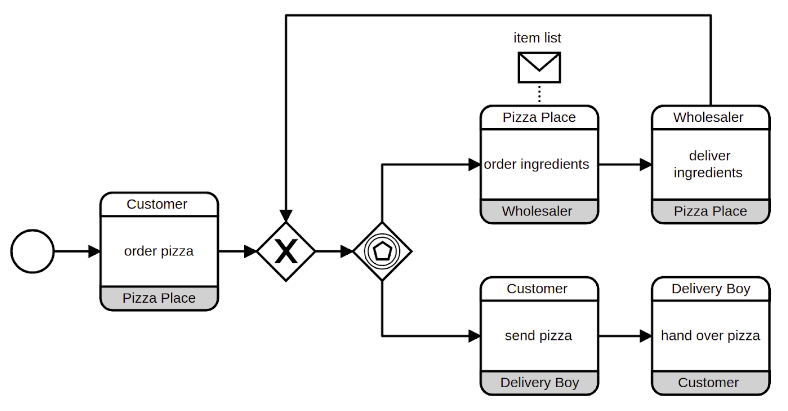
\includegraphics[scale=0.6]{bpmn.png}
    \caption{Choreography diagram of a pizza ordering process} 
    \label{fig:simple_bpmn}
\end{figure}


Throughout this paper we will try to present our thoughts in more concrete fashion by applying them to the example shown in \reffig{fig:simple_bpmn}. Here the parties are collaborating without trust (\ber{a}, \ber{b} and \ber{c}). They also have an urge to keep as much as possible about their collaboration secret (\ber{d}, \ber{e} and \ber{f}). An example of \ber{g} and \ber{h} would be that the \textit{D} \todo{Could you please make a version with capitalized abbreviations? E.g. Delivery Boy to D.}
 should not know anything about the collaboration between \textit{W} and \textit{P}, even though he is part of the overall business process. 



\subsection{Proposed Schema} \label{subsec:schema}

In this chapter we discuss our proposed schema. We will do so by introducing mechanisms which each solve one or more of the premises of \refsec{subsec:assumptions} \todo{section x will combine all mechanisms}.

\bigbreak
\textbf{Circles.} In order to solve problem \ber{g} and (in part) \ber{h}, we introduce the notion of circles. Circles are visibility constraints for a group of entities. A message exchanged within a circle can only be read by other participants of a circle. We achieve this by using symmetric keys which are exchanged between the members of a circle before the execution of the process. This can be done by using established processes like \todo{openPGP? Find source!}. Which parties are within which circle should be established by the parties themselves and is thus out of scope of this paper. \ref{fig:circles} shows an example of possible circles of the process defined in  \reffig{fig:circles}. Each circle has its own associated symmetric key and each message is encrypted with that key. This way \ber{D} cannot read the communication between \ber{W} and \ber{P}. Also the message can still be included in the audit trail, since only \ber{W} and \ber{P} can read it. This encryption also keeps the \ber{Content Layer} of the process secret (premise \ber{f}).

\begin{figure}[h!]
    \centering
    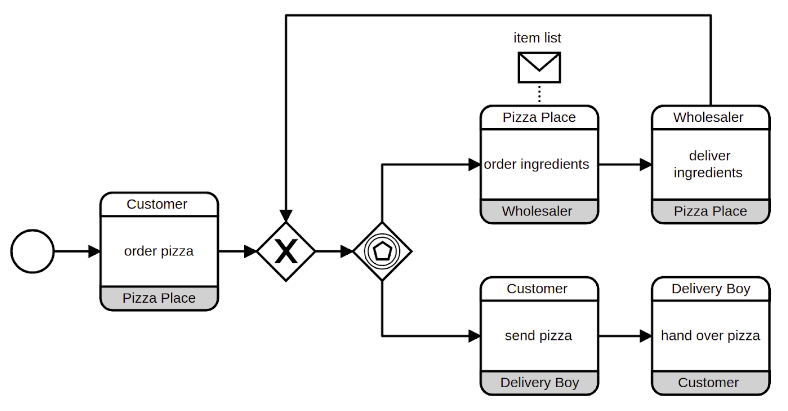
\includegraphics[scale=0.6]{bpmn.png}
    \caption{Circles for of the process described in \reffig{fig:circles}} 
    \label{fig:circles}
\end{figure}

\todo{write abbreviation in the illustration}


\bigbreak
\textbf{Protecting the Model Layer.} Since we consider all communication and all code execution on the blockchain as public (premise \ber{i}), we decided to store and execute the logic off-chain. This is in order to keep the \ber{Model Layer} secret (premise \ber{d}). The representation of the business process is shared amongst all entities. This could be a graph or executable code. This representation should vary in detail, hiding the details of the process that are out of the own circle. How this representation looks like exactly and how it is shared is out of scope of this paper.


\bigbreak
\textbf{Enforceability.} sdndlj





\section{Evaluation} \label{sec:eval}

implementation


\section{Discussion} \label{sec:discussion}

\begin{itemize}
    \item shortcomings
    \item How could mentioned in \refsec{subsec:technologies} improve \refsec{sec:eval}?
    \item How did it work out in the end? 
    \item private blockchain
    \item Parity
    \item future work
\end{itemize}


\section{Conclusion} \label{sec:conclusion}

final words




\bibliographystyle{splncs04} % BibTeX users should specify bibliography style 'splncs04'.
\bibliography{refs} % Entries are in the "refs.bib" file


\end{document}
